  \documentclass[twoside=false, %  doppelseitiger Druck
    DIV=15,% DIV Faktor für Satzspiegelberechnung, sie Doku zu KOMA Script
    BCOR=15mm, % Bindekorrektur
    chapterprefix=false,
    headinclude=flase,
    footinclude=false,
    pagesize,%         write pagesize to DVI or PDF
    fontsize=11pt,%             use this font size
    paper=a4,%          use ISO A4
    bibliography=totoc,%         write bibliography-chapter to table of contents
    index=totoc,%         write index-chapter to table of contents
    cleardoublepage=plain,% \cleardoublepage generates pages with pagestyle empty
     headings=big,%       A4/B5
    listof=flat,%        improved list of tables
    numbers=noenddot
  ]{scrbook}

\usepackage[
a4paper,% other options: a3paper, a5paper, etc
left=3cm,
right=2cm,
top=2cm,
bottom=2cm,
% use vmargin=2cm to make vertical margins equal to 2cm.
% us  hmargin=3cm to make horizontal margins equal to 3cm.
% use margin=3cm to make all margins  equal to 3cm.
]
{geometry}
\usepackage[utf8]{inputenc}
\usepackage{makeidx}
\usepackage{acronym}
\usepackage{amsfonts}
\usepackage[slantedGreek,sc]{mathpazo}  % Schriftart Palatino
% \usepackage{lmodern}    % statt mathpazo, falls CM Fonts verwendet werden sollen
%\usepackage{mathptmx}    % statt mathpazo, falls Times  verwendet werden soll
\usepackage[scaled=.95]{helvet}
\usepackage{courier}
\usepackage[T1]{fontenc}
\usepackage{textcomp}
\usepackage{amsmath}            % standard math notation (vectors/sets/...)
\usepackage{bm}        % standard math notation (fonts)
\usepackage{fixmath}        % standard math notation (fonts)
\usepackage{graphicx}
\usepackage[facing=yes]{floatrow}       % mehrere Gleitobjekte nebeneinander/caption neben Bild/Tabelle
\usepackage[labelfont=bf,sf,font=small,labelsep=space,format=plain]{caption}
\usepackage{subcaption}
\usepackage{scrlayer-scrpage}
% \usepackage{pstool}  % einbinden falls psfrag verwendet werden soll
\usepackage{epstopdf}
\usepackage[ngerman]{babel}
\usepackage{ellipsis}  % Korrigiert den Weißraum um Auslassungspunkte
\usepackage{microtype}  % optischer Randausgleich etc.

\usepackage{xcolor}         % z.B. für schattierte Boxen
\usepackage{framed}			% shaded Umgebung
\usepackage{setspace}		% für den Zeilenabstand
\definecolor{shadecolor}{gray}{.85}%

% Links im PDF
\usepackage[colorlinks=false,
            pdfborder={0 0 0},
            breaklinks=true]
            {hyperref}
\usepackage{pdfpages}
%\usepackage{biblatex}
%\typearea[current]{calc}


% Einstellungen für Bild-/Tabellenbeschriftung neben dem Bild
\floatsetup[figure]{capbesideposition={inside,top}}
\floatsetup[table]{capbesideposition={inside,top},style=plaintop}
\renewfloatcommand{fcapside}{figure}[\capbeside][\FBwidth]
\newfloatcommand{tcapside}{table}[\capbeside][\FBwidth]


\selectlanguage{ngerman}


\deffootnote{1em}{1em}{%
 \makebox[1em][l]{\thefootnotemark}}

\makeindex

\newcommand{\real}{\mathord{\mathrm{I\!R}}}

% Kapitel starten auch auf selber Seite
\usepackage{etoolbox}
\makeatletter
\patchcmd{\scr@startchapter}{\if@openright\cleardoublepage\else\clearpage\fi}{}{}{}

\makeatother

\begin{document}
\selectlanguage{ngerman}
\def\figdir{figures}
\def\tabledir{tables}

\frontmatter

\pagestyle{scrplain}
\pagestyle{empty}

\begin{titlepage}

\sffamily

\raggedleft

\vspace*{-2cm}


\includegraphics{\figdir/logo-th-rosenheim-2019_master_quer_2c.eps}

\vfill

\centering
\LARGE
% \vspace*{\fill}
%-----------
Fakultät für Informatik  \vspace{0.5cm}\\
\Large
Studiengang Informatik

\vspace{2cm}

\LARGE

DevSecOps mit Azure DevOps Pipelines und GitHub Actions

\vspace{2cm}

\Large
Projektarbeit im Fachwissenschaftlichen Wahlpflichtmodul DevOps

\vspace{1.5cm}


\Large
von

\vspace{0.5cm}

%\vspace*{\fill}

\LARGE
Florian Weidner \vspace{1cm}

\vspace{1cm}

\flushleft
 \Large
\vspace*{\fill}

%-----------
\begin{tabbing}
Datum der Abgabe: \= tt.mm.jjjj \kill
Datum der Abgabe: \> tt.mm.jjjj \\
Prüfer: \> Daniel Kerschagl \\

\end{tabbing}
%-----------

\end{titlepage}
%\cleardoubleemptypage
%\chapter*{Kurzfassung}
\thispagestyle{empty}
text

\bigskip

\noindent
Schlagworte: 


%\cleardoubleemptypage

\pagestyle{scrplain}
\pagenumbering{roman}
% ---------------------------------------------------
% D-TOC.TEX zur Verwendung mit TEXPART
% (an eigene Gegebenheiten anzupassen)
% ---------------------------------------------------
%
\tableofcontents
\clearpage
\listoffigures
%\clearpage
%\listoftables
%\cleardoublepage


\pagestyle{scrheadings}


\addtokomafont{caption}{\small}

\mainmatter

\onehalfspace
\chapter{Firmenbeschreibung}
\section{ORCA Software GmbH}
Die ORCA Software GmbH wurde im Jahr 1990 von Dipl.-Ing. Siegfried Tille und Dipl.-Ing. Heinz Nießen gegründet. Der Hauptsitz des Unternehmens ist in Neubeuern Nähe Rosenheim. Das Unternehmen entwickelte, vertreibt und supportet Software spezialisiert mit dem Ziel, die Ausschreibung, Vergabe und Abrechnung für Bauingenieure, Architekten und Bauplaner zu vereinfachen. Hierfür bietet die ORCA Software GmbH die Desktopanwendungen ORCA AVA, ORCA OBJEKT, ORCA TEXT und auch die Website AUSSCHREIBEN.DE an. Der Leitgedanke war und ist eine Software zu entwickeln, welche für jedermann verständlich ist. \cite{Orca} 

\section{ORCA \ac{ava}}
Die ORCA \ac{ava} ist für alle Architektur- und Ingenieurbüros, Wohnungsbaugesellschaften, Unternehmen und Behörden zur einfachen Abwicklung von Bauprojekten mit Ausschreibung, Vergabe und Abrechnung. Auch das Kostenmanagement von solchen Projekten lässt sich in der Software ideal umsetzen. Des Weiteren unterstützt die Bausoftware alle Leistungsphasen der \ac{hoai} und unterstützt zudem \ac{bim}. Das Programm stellt diverse DIN zertifizierte Schnittstellen für den einfachen Austausch und Import oder Export von Dateien bereit. Das Hauptziel ist eine einfach verständliche Software, welche intuitiv und klar zu bedienen ist, an den Kunden zu bringen. Es stehen drei verschiedene Editionen zur Auswahl. Die ORCA \ac{ava} Starter Edition SE, Professional Edition PE und die Enterprise Edition EE. Im April 2022 erscheint die neueste Version ORCA \ac{ava} 25.0.

\section{ORCA OBJEKT}
Die ORCA OBJEKT ist eine Bausoftwarelösung für das Objektgeschäft. Sie dient als unterstützendes Tool zur zentralen Datenpflege und bei der Erstellung von individuellen Leistungsverzeichnissen. Zudem ermöglichen zahlreiche Standardschnittstellen einen sicheren Datenaustausch.

\section{ORCA TEXT}
Die Software ORCA TEXT ist die Grundlage für die Website AUSSCHREIBEN.DE. Sie ermöglicht es Produktherstellern einfach und intuitiv Ausschreibungstexte für ihre Produkte zu erstellen. Diese Texte können über die Software verwaltet und anschließend in der Website übernommen werden. 

\section{AUSSCHREIBEN.DE}
AUSSCHREIBEN.DE verfügt über 1 Millionen Ausschreibungstexte von über 600 Herstellern aus verschiedenen Gewerken. Es ist eine wichtige Bezugsquelle für Architekten, Bauingenieure und Planer bei der Ausschreibung ihrer Bauvorhaben.

\chapter{Arbeitsumfeld und Vorgeschichte}

\section{Vorgeschichte Verbundstudium}
Das Praxissemester startete Offiziell am 01.09.2021. Durch mein Verbundstudium arbeite ich aber schon seit September 2018 bei der ORCA Software GmbH und auch die Praxisphase startete direkt nach den Prüfungen des vierten Semesters. Das erste Jahr meines Verbundstudiums habe ich in der Qualitätssicherung, die Grundlagen des Programmierens, das Unternehmen und die Produkte näher kennengelernt. Gleichzeitig mit dem Studienstart wechselte ich ab Herbst 2019 ins  AUSCHREIBEN.DE Entwicklungsteam und habe dort viele praktische Erfahrungen gesammelt. Ich habe dort sowohl am Frontend und am Backend bei der Neuentwicklung von AUSCHREIBEN.DE mitgearbeitet. Mit dem Start des Praxissemesters wechselte ich in das \ac{ava} Entwicklungsteam. Beim Wechsel wurden mir meine Aufgaben und Projekte für das Praxissemester mitgeteilt. Durch mein Verbundstudium hatte ich zusätzlich während der Praxisphase noch eine Projektarbeit, eine schriftliche und eine mündliche Abschlussprüfung meiner Ausbildung. Das Schreiben und Lernen wurde dem Arbeiten im Entwicklungsteam vorgezogen.

\section{Arbeitsumfeld}
Die Entwicklung ist getrennt in zwei Entwicklungsteams, der ORCA \ac{ava} und AUSSCHREIBEN.DE. Mit der Entwicklung der ORCA \ac{ava} sind etwa 10 Personen beauftragt. Die meisten Entwickler arbeiten an neuen Features der zukünftigen ORCA \ac{ava} Version. Am Anfang war das für die 24.1, die im November 2021 freigegeben wurde, und anschließend für die Version 25, die im April 2022 erscheinen soll. Einige Entwickler sind auch mit der Ablösung des \ac{vb6} Codes beschäftigt, indem die ORCA \ac{ava} noch im Kern programmiert ist. Diese Arbeiten sind oft für Kunden und in der Oberfläche nicht zu erkennen, kosten aber viel Entwicklungsaufwand.

Das Team arbeitet mit SCRUM in zweiwöchentlichen Sprints. Es findet jeden Tag ein Daily statt, um den aktuellen Entwicklungsstand bei allen Entwicklern zu synchronisieren.
Als Konfigurationsmanagement Tool wurde ein Team Foundation Server mit DevOps benutzt.
Beim Sprint Planning, dass alle zwei Wochen stattfindet, werden Ziele für den nächsten Sprint definiert. Diese werden dann in Userstories mit Anforderungen in DevOps erstellt und dem Sprint zugewiesen. Danach unterteilt jeder Entwickler seine Userstories in Tasks und schätzt den Zeitaufwand. Beim Abarbeiten, werden die Tasks auf dem SCRUM Board auf aktiv und am Ende auf geschlossen gesetzt, sodass jeder Entwickler einsehen kann, welche Aufgaben andere gerade bearbeiten. Außerdem wird beim Checkin die Task-Id angehängt, um das jeweilige Arbeitselement automatisch zu schließen. Dadurch kann jeder die Entwicklungshistorie zurückverfolgen und auch als Dokumentation nutzen.

Die Aufgaben und Anforderungen kamen vom \ac{ava} Entwicklungs-Teamleiter Günter Holzeder, welcher mir Anfangs auch als Projektbetreuer zur Verfügung stand. Die Projektbetreuung wurde später von einem anderen Senior Developer abgenommen.

\chapter{Projekt \ac{ava} Manager}

\section{Projektrahmen und Umfeld}

Die ORCA \ac{ava} soll einen neuen Startdialog bekommen. Für das Projekt wurde mir anfangs ein eigener Feature-Branch erstellt. Auf dem Hauptbranch, dem sogenannten "trunk", läuft beim Einchecken ein Gated-Checkin der die Lauffähigkeit des Codestandes überprüft. Dieser Gated-Checkin auf der Build-Maschine ist noch nicht mit .NET 6 kompatibel. Deswegen konnte ich diesen nicht benutzen. Auf  Feature-Branchs laufen allerdings standardmäßig keine Gated-Checkins, wodurch ich die meinen .NET 6 Code versionieren konnte.

\section{Ausgangspunkt}
Im Moment erscheint beim Start der ORCA \ac{ava} ein klassischer „Datei öffnen“ Dialog. In diesem kann man seine .ava Projektdatei einlesen und sein Bauprojekt lokal oder im Firmennetzwerk bearbeiten. 

Die aktuelle ORCA \ac{ava} ist in zwei verschiedenen Sprachen implementiert. Der Rumpf besteht aus \ac{vb6} Code und Forms als Frontendframework, während neuere Komponenten in C\# und WPF entwickelt wurden. Die Software läuft somit nur auf Windows. Da \ac{vb6} schon alt ist, werden von Zeit zu Zeit Komponenten durch C\# abgelöst. In diesem Zuge soll auch der Startdialog neu implementiert werden.

\section{Anforderungen und Ziel}
Bei der stückweisen Ablösung von \ac{vb6} Code kann auch fachlich einiges angepasst werden, da die Komponenten komplett neu programmiert werden müssen.
Beim Ablösen des Startdialog soll der sogenannte \ac{ava} Manager entstehen. In diesem kann man seine verschiedenen Bauprojekte dateiunabhängig auswählen und starten. Zusätzlich kann man aber auch z.B. Lizenzen verwalten, Updateinformationen erhalten oder weitere projektübergreifende Einstellungen tätigen. Dadurch werden die Projektfenster schlichter, fokussieren sich nur noch auf ein Projekt und es können auch mehrere \ac{ava} Projekte gleichzeitig geöffnet werden. Außerdem müssen Projekte nicht mehr lokal im Dateisystem existieren. Es entsteht dadurch eine Dateiunabhängigkeit und Projekte können zum Beispiel auch in einem Cloud-Storage liegen.

Für den \ac{ava} Manager wird eine passende Frontend-Technologie gesucht. Technologisch ist der \ac{ava} Manager unabhängig, da er eine ORCA \ac{ava} Instanz in einem neuen Prozess startet. Es stehen allerdings schon viele grundlegende .NET Bibliotheken der ORCA \ac{ava} zur Verfügung. Es sollte also ein Framework aus dem .NET Stack sein. Meine Aufgabe war es die neue Technologie .NET \ac{maui} Blazor als Möglichkeit für den \ac{ava} Manager zu untersuchen.
Dazu sollte zusätzlich das Framework Telerik UI for Blazor verwendet werden. Telerik bietet fertige Oberflächenkomponenten an, um die Entwicklungsgeschwindigkeit zu steigern.
Die Anforderungen waren am Anfang, dass ein Testprojekt entstehen soll, welcher als erster Prototyp für den \ac{ava} Manager dient. Es sollten möglichst viele verschiedene Kontrollelemente von Telerik eingebaut werden, um einen Überblick über die Möglichkeiten des Frameworks zu bekommen. Ein weiterer Punkt war die Barrierefreiheit. Die Technologien sollen hier anerkannte Standards erfüllen.

Im Laufe des Projektes kamen immer mehr Anforderungen hinzu. Durch die Recherche und das angesammelte Wissen entstanden neue Probleme, aber auch Möglichkeiten die zu neuen Aufgaben führten. Nachdem der \ac{gui}-Klickdummy fertig war, sollte vor allem das TreeList-Control von Telerik genauer untersucht werden, da Bäume ein zentrales Element in der ORCA \ac{ava} sind. In Abbildung \ref{fig:LV-der-AVA} ist zu sehen, dass komplette Projektstruktur in einem Baum abgebildet wird.

Das TreeList-Control sollte auch über diese Features verfügen und dem ORCA \ac{ava} Baum nachimplementiert werden. 
Auch als das Beispiel des TreeList-Controls erstellt wurden boten sich neue Möglichkeiten an und es entstand der Wunsch einen \ac{ava}-Baum mit echten Daten zu befüllen. Die Oberfläche sollte also mit dem Data Provider, der Datenzugriffsschicht der ORCA \ac{ava} kommunizieren und ein Leistungsverzeichnis angezeigt werden.

\section{Recherche und Einarbeitungsphase zu den Technologien}

Die Ergebnisse wurden in Microsoft Teams in einer Präsentation festgehalten und dokumentiert.

\subsection{.NET \ac{maui}}
Die Recherche zu .NET \ac{maui} Blazor stellte sich teilweise als schwierig heraus. Die Technologie ist noch in der Preview Phase und es existierte anfangs fast keine Dokumentation von Microsoft. Dadurch fand man auch wenig Erklärungen, Beispiele und Tutorials von anderen Portalen. Auf der Seite von Microsoft wird viel Werbung gemacht mit „cross platform“ oder „single shared codebase“. Auch der Begriff „Blazor Desktop“ wurde auf IT-News Seiten und Blogs oft genannt. Diese Begriffe musste ich zuerst einzuordnen und sortieren, um zu verstehen, was das besondere und neue an dem Framework ist.

Es ist wichtig, das man zwischen zwei Möglichkeiten unterscheidet. Es gibt einerseits die standardmäßige .NET \ac{maui} Applikation bei der, wie auch schon der Vorgänger Xamarin, die Oberfläche mit XAML programmiert wird. Andererseits gibt es eine .NET \ac{maui} Blazor App, bei der die \ac{gui} mit .NET Blazor implementiert wird. Am Start des XAML Codes ist hier ein BlazorWebView Element (siehe Abbildung \ref{fig:blazor-integration}), das auf der Technologie WebView2 basiert. Somit wird .NET Blazor nativ eingebunden. Im .NET Stack gab es davor keine Möglichkeit Desktopanwendungen mit HTML und CSS zu programmieren. \cite{Davidbritch_22}


\subsection{.NET Blazor}
.NET Blazor ist ein Webframework für .NET Entwickler, das C\# in binäres WebAssembly kompiliert. Diesen Code kann ein Browser dann verstehen und direkt ausführen. Wenn man aber damit klassische Websites programmiert, hat man keine Möglichkeit lokale Ressourcen wie Dateien oder Registry-Einträge zu verwalten. In einer .NET \ac{maui} Applikation läuft der Code nativ und ermöglicht es der Blazor-Oberfläche auf lokale Ressourcen zuzugreifen und diese Anzuzeigen.
Es stellte sich heraus das vor allem die Technologie .NET Blazor zum Entwickeln des \ac{ava} Managers nötig ist und .NET \ac{maui} nur einen Rahmen bietet den HTML Code nativ laufen zu lassen. In Abbildung \ref{fig:blazor-integration} ist der XAML-Tag BlazorWebView zu sehen, welches diesen Rahmen für den Blazor Code bietet. Durch meine guten Kenntnisse HTML, CSS und C\# war die Einarbeitung in .NET Blazor einfach. Auch durch meine Kenntnisse in Angular, die ich schon im AUSSCHREIBEN.DE Team gesammelt habe, wusste ich wie ein solches Webframework funktioniert und habe viele konzeptionelle Strukturen wiedererkannt.

\begin{figure}[h]
	\centering
	{\caption{Code der Blazor Integration im MainPage.xaml}
		\label{fig:blazor-integration}}
	{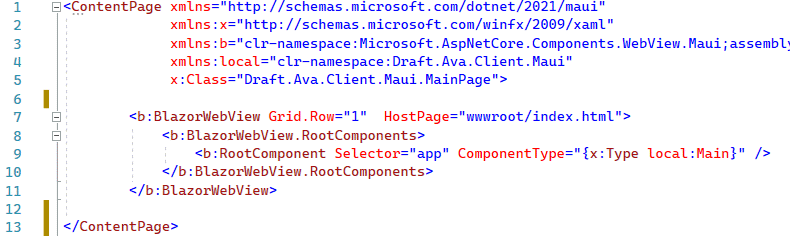
\includegraphics[width=1\textwidth]{\figdir/blazor-integration}}
\end{figure}

\subsection{Telerik UI for Blazor}
Mit dem externen Komponenten-Framework Telerik UI for Blazor hatte ich zuvor auch noch keinen Kontakt und keine Erfahrungen. Das Einarbeiten war allerdings sehr kurzweilig und einfach. In der Dokumentation gibt es eine gute Übersicht über alle verfügbaren Elemente. Zu jedem Control gibt es dann verschiedene Demobeispiele mit passendem Code und eine zusätzliche Dokumentation mit den Eigenschaften und Möglichkeiten der Komponente. Auch das Einbinden in ein .NET Blazor Projekt wurde beschrieben und geschildert, was auch das integrieren in die .NET \ac{maui} Blazor App einfach gemacht hat.
Für meine Untersuchungen wurde mir extra eine neue Entwicklerlizenz bereitgestellt, um das Framework wirklich testen zu können. Die Lizenz wurde für 899€ bestellt und mir zugewiesen. \cite{Telerik_22}

\section{Erstellen eines Prototypen}

\subsection{Erstellen eines Prototypen}
\label{chap:create-prototype}
Durch die mäßig erfolgreiche Recherche zu .NET \ac{maui}, startete ich mit dem Entwickeln eines Testprojekt. Durch die fehlende Dokumentation, gab es anfangs viele Probleme und Startschwierigkeiten. Um ein .NET \ac{maui} Projekt anzulegen brauchte man eine spezielle Preview-Version von Visual Studio und auch noch einige zusätzliche Software, die installiert werden mussten. Durch die .NET \ac{maui} Blazor Vorlage im Visual Studio war das Anlegen kein Problem. Aufgrund der Preview-Version konnte man das Projekt allerdings nicht direkt starten oder debuggen. Man musste es immer zuerst auf dem lokalen Rechner deployen, um es dann starten zu können. So entstand nach 2 Wochen ein \ac{gui}-Dummy (siehe Abbildung \ref{fig:layout-manager}), der viele Telerik-Komponenten enthielt und einem Vorschlag aus der Produktdesign Abteilung nachimplementiert war. In dieser Version wurden alle ursprünglichen Anforderungen umgesetzt. 

\begin{figure}[h]
	\centering
	{\caption{Code der Blazor Integration im MainPage.xaml}
		\label{fig:layout-manager}}
	{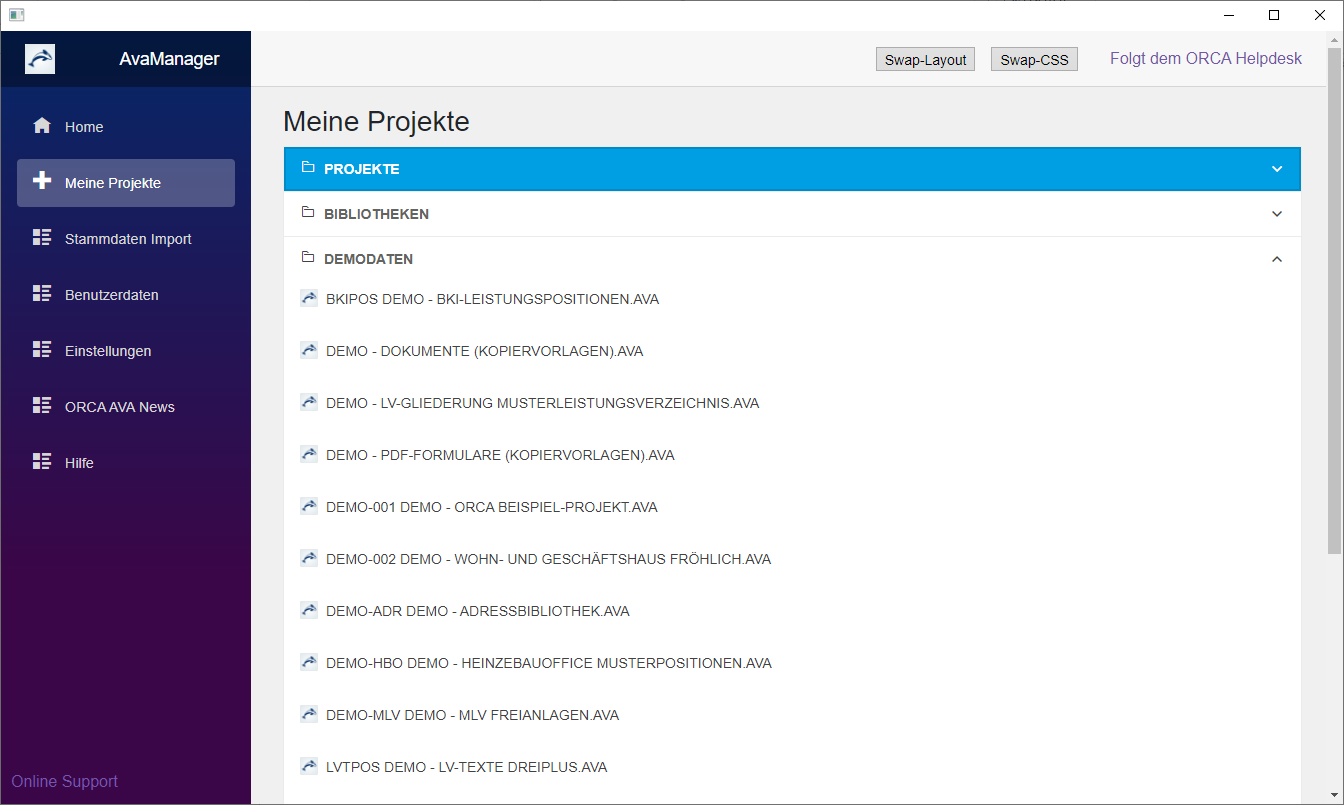
\includegraphics[width=1\textwidth]{\figdir/layout-manager}}
\end{figure}

\begin{figure}[h]
	\centering
	{\caption{Vergleich zwischen Button in Blazor (links) und Forms (rechts) }
		\label{fig:css-example}}
	{
\includegraphics[width=1\textwidth]{\figdir/css-example}}
\end{figure}

Ein Dateisystemzugriff sowie das Starten weiterer ORCA \ac{ava} Prozesse sollte veranschaulichen, dass es ich um eine native Applikation handelt. Dies lies sich ohne Probleme umsetzten und der Blazor-Code konnte direkt diese Systemaufrufe ausführen.
Der Stiel des \ac{ava} Managers konnte zwischen dem ORCA \ac{ava} Design und dem ORCA Telerik Design per Button gewechselt werden. Die Telerik Komponenten nutzen ein globales CSS-File mit rund 37.000 Zeilen, dass das Design der Elemente definiert. Dieses habe ich kopiert und an einigen Stellen angepasst um den Stil der ORCA \ac{ava} nachzuahmen. Durch meine CSS Kenntnisse war dies leicht umzusetzen und das Ergebnis war nahe am Original. In Abbildung \ref{fig:css-example} sieht man den Vergleich am Beispiel eines Buttons. Es wurden Farben, Umrandungen, Schriftart und Größe angepasst.
Durch die Nachahmung, sollen die Kunden keine Stilbrüche erleben und wenn man das Design modernisieren will, ist dies auch durch die zentrale Implementierung leicht umzusetzen.
Somit war der erste Prototyp fertig, und das Nutzen von .NET Blazor als Frontendtechnologie hat sich für den \ac{ava} Manager und auch weiterer Komponenten bestätigt.

\subsection{Untersuchen des TreeList Controls}
Obwohl das TreeList-Control von Telerik keine wichtige Funktion im \ac{ava} Manager haben wird, sollte es genauer untersucht werden, da es für die ORCA \ac{ava} generell eine sehr wichtige Bedeutung hat. Die Baumstruktur der ORCA \ac{ava} hat viele Funktionen. Diese sollten das Telerik TreeList-Control auch können. Es war das Ziel diese Funktionen auch im Testprojekt zu implementieren um herauszufinden ob diese realisierbar sind.
Ich habe zuerst den ORCA \ac{ava} Baum analysiert und die wichtigsten Eigenschaften dokumentiert. (siehe Abbildung \ref{fig:tree-requirements}) Diese wurden dann mithilfe der Telerik Dokumentation in eine der ORCA \ac{ava} nachgeahmten Baum im Testprojekt integriert. Das TreeList-Control konnte fast alle Funktionen abdecken. Die meisten mussten bloß über Eigenschaften des Controls konfiguriert werden. Einzig das Reihen-bezogene Kontextmenü konnte nicht optimal umgesetzt werden. Das Problem wird in \autoref{chap:external-components} genauer beschrieben.

\begin{figure}[h]
	\centering
	{\caption{Anforderungen an das Telerik TreeList-Control }
		\label{fig:tree-requirements}}
	{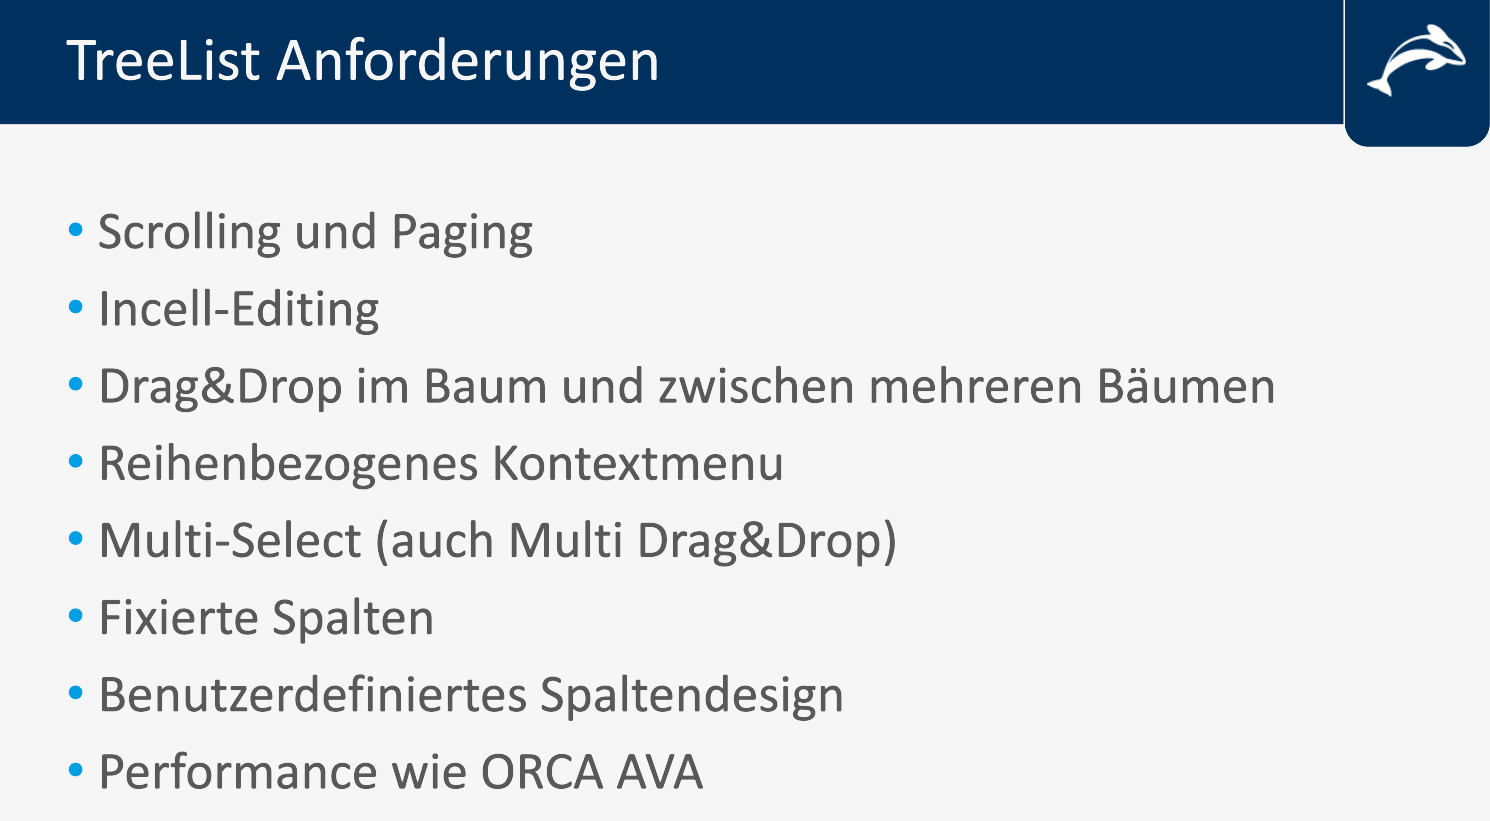
\includegraphics[width=1\textwidth]{\figdir/tree-requirements}}
\end{figure}

\subsection{Anbinden an die vorhandene Datenzugriffsschicht}
Nachdem die Funktionalität des Kontrollelements getestet wurden, entstand der Wunsch einen mit echten Daten befüllten \ac{ava} Baum zu implementieren. Die Datenzugriffsschicht in der ORCA \ac{ava} ist der sogenannte DataProvider. Dieser läuft in einem eigenem Prozess und ist lokal über \ac{http} erreichbar. Die .NET \ac{maui} App soll auf den DataProvider zugreifen, welcher eine .ava Datei ausließt und eine Leistungsverzeichnis zurückgibt. Bei der Planung stoß ich schnell auf Probleme mit den Framework-Version. Der .NET Code der ORCA \ac{ava} ist seit kurzen auf .NET Framework 4.8. Darunter auch der DataProviderClient welcher als Client zur Kommunikation mit dem DataProvider für den \ac{ava} Manager benötigt wäre. Da .NET \ac{maui} nur mit der Preview-Version von .NET 6 läuft, musste das Framework des DataProviderClient mit seinen Abhängigkeiten angehoben werden. Bei der Umstellung hatte ich Unterstützung von einem weiteren Entwickler, der schon Erfahrung mit Frameworkumstellungen hat. Er erklärte mir die grundlegende Vorgehensweise und Punkte die dich beachten sollte.
Die Umstellung umfing 12 Projekte die aktualisiert werden mussten. Mit der Frameworkversion änderte sich auch die Struktur der Projektdateien. Ein weiterer Entwickler hatte diese allerdings schon mit dem Update von .NET Framework 4.7 auf 4.8 auf die aktuelle Struktur angepasst. Somit habe ich Projekt für Projekt die Version angehoben bis der DataProviderClient auf .NET 6 Buildfähig war. Damit konnte der Code auch aus dem \ac{ava} Manager aufgerufen werden. Beim Testen der Anwendung stürzte diese allerdings bei der Datenabfrage ab.

Durch die Frameworkumstellung entstand ein Bug bei der Kommunikation mit dem DataProvider. Diese läuft über \ac{owin}, dem damaligen Standard .NET Interface für Webserver und Webanwendungen. \ac{owin} benutzt \ac{http} und Nachrichten werden mit Json serialisiert. Dazu wird im DataProviderClient das weit verbreitete Nuget-Package Newtonsoft.json benutzt. Hier wurden die Daten durch die Frameworkumstellung bei der Serialisierung eines Objekt-Arrays anders abgebildet als noch mit der alten Version. Dadurch hatte sie der DataProvider in eine andere Objektstruktur deserialisiert und landete in einem Fehler. Dieser Fehler war sehr schwer zu identifizieren und es dauerte lange bis ich ihn mit einem Workaround behoben konnte.

Somit funktionierte dann die Datenübernahme aus dem DataProvider. Es musste noch die Datenstruktur des TreeList Controls auf die Struktur des DataProviders abgebildet werden. Am Ende konnten dann reale \ac{ava} Daten in der Oberfläche angezeigt werden (siehe Abbildung \ref{fig:tree-result}).

\section{Abnahme und Vorstellung}
Zwischenstände und interessante Erkenntnisse wurden regelmäßig mit dem \ac{ava} Entwicklungs-Teamleiter kommuniziert. Außerdem wurden Zwischenstände des entstandenen Prototypen in den Sprint Reviews vorgestellt, um auch den anderen Entwicklern einen Einblick über das entstandene Projekt zu geben.
Das Endergebnis des Prototypen wurde zusätzlich vom Teamleiter am ORCAner Tag vor allen Mitarbeitern vorgestellt. An diesem Tag wurden den Mitarbeitern die Planung für die nächsten Jahre von der Geschäftsführung und den Teamleiter geschildert und begründet. Bei der Zukunftsplanung der ORCA \ac{ava} wurde dabei mein Projekt vorgestellt. Es wurde demonstriert wie der \ac{ava} Manager aussehen könnte und mit dem implementierten Leistungsverzeichnis mit realen Daten die Möglichkeiten von .NET Blazor gezeigt.

\section{Projektfortführung und Ausblick}
Nach dem Anbinden des DataProviders und der Präsentation am ORCAner Tag wurde vom Teamleiter entschieden, das erstmals genug Informationen gesammelt wurden. Es muss vor allem auf den .NET \ac{maui} Release im 2 Quartal 2022 gewartet werden um mit der Entwicklung richtig starten zu können. Der \ac{ava} Manager soll in der Version 26 entstehen. .NET Blazor ist nach der Analyse der Hauptkandidat als Frontend-Technologie. Es stellte sich heraus, dass man Blazor seit dem .NET 6 Release auch in \ac{wpf} Projekt einbinden kann. Diese Möglichkeit steht neben .NET \ac{maui} für die Entwicklung auf dem Plan. Um Blazor in WPF einbinden zu können, muss der ganze \ac{ava} Code auf der aktuellsten Frameworkversion .NET 6 sein. Diese Umstellung soll als nächstes Angestoßen werden um solche neuen Möglichkeiten nutzen zu können.



%%%%%%%%%%%%%%%%%%%%%%%%%%%%%%%%%%%%%%%%%%%%%%%%%%%%%%%%%%%%%%%%%%%%%%%%%%%%%%


\chapter {Kurzbericht: Folgeprojekt .NET 6 Umstellung}
Im laufe der Recherche zum \ac{ava} Manager wurde klar, das die Umstellung auf .NET 6 viele Möglichkeiten für die Zukunft bietet. Außerdem sollte der Codestand immer möglichst zeitnah auf die aktuelle Version gehoben werden. Nachdem das Projekt für den \ac{ava} Manager fertig war, bekam ich die Aufgabe die Umstellung auf .NET 6 zu untersuchen und anzustoßen. Bei einem Kickoff Meeting mit einigen Entwicklern wurde festgelegt, dass die einzelnen Prozesse der ORCA \ac{ava} Schritt für Schritt umgestellt werden sollen. Der DataFormatsBrowser, einem eigenem Prozess für die Datenübernahme in die ORCA \ac{ava}, sollte zuerst umgestellt werden. Hierfür wurde eine eigene Solution erstellt. Diese kann auf .NET 6 umgestellt werden, ohne das der restliche Entwicklungsbetrieb etwas davon mitbekommt, ich aber auf dem Hauptentwicklungsbranch bleiben kann. Mit einer neuen Konfigurationsdatei kann man die Frameworkversion der einzelnen Projekte in den verschiedene Solutions konfigurieren. Ich habe dann alle Abhängigkeiten und Nuget-Packete untersucht um die nicht mit .NET 6 kompatibel Komponenten zu finden. Wenn Pakete noch nicht mit dem neuen Framework funktionieren, habe ich nach Lösungen dafür gesucht. Für den DataFormatsBrowser musste eine wichtige externe Komponente aktualisiert werden. Diese Arbeit vollzog der Entwickler, der diese Komponente integriert hat.
Danach begann die testweise Umstellung auf die neue Frameworkversion. Nachdem Projekt für Projekt umgestellt und lauffähig war habe ich das Programm getestet und keine Fehler festgestellt. Die Datenübernahmen haben normal funktioniert. In meiner restlichen Zeit der Semesterferien sollen entstandene Build-Warnungen entfernt, der Gated-Checkin angepasst und die Unittests mit umgestellt werden.

\chapter{Faktoren zum Projekterfolg/-misserfolg}

\section{Previewstatus des Frameworks .NET \ac{maui}}
Ein Framework im Previewstatus ist natürlich noch nicht fertig und kann noch viele Fehler enthalten. Am Anfang des Projektes waren die Einschränkungen mit den ersten Preview-Versionen des Frameworks sehr hoch. Am meisten Probleme hat mir die fehlende Dokumentation gemacht. Microsoft bieten generell sehr umfangreiche und übersichtlicher Anleitungen und Codedokumentationen an, die ich in der Vergangenheit oft benutzt habe. Bei .NET \ac{maui} beschränkte sich diese anfangs auf einer Erklärung und einem "Get Started". Das Anlegen eines solchen Projektes war durch diese Anleitung einfach umzusetzen. Als die Projektvorlage angelegt war und man das Projekt einmal gestartet hat, musste man zuerst alleine die Projektstrukturen und den erstellten Code selber verstehen. Es wurden keine weiteren Informationen dazu bereitgestellt.

Einige Bugs im Zusammenhang mit der Preview-Version von Visual Studio haben auch die Entwicklungsgeschwindigkeit reduziert. Neben dem bereits in \autoref{chap:create-prototype} schon beschriebenen fehlendem Debugging gab es auch weitere Probleme bei der Preview-Version. Es wurde circa monatlich eine neue Preview-Version veröffentlicht. Mit jeder neuen Version nahm die Anzahl an Fehlern ab, das Migrieren des Projektes hat aber oft nicht einwandfrei geklappt. Durch Änderungen zum Beispiel an der Projektstruktur musste ich immer wieder neue Projekte anlegen und den Code selber kopieren und teilweise auch wieder anpassen. Ein konkretes Beispiel war, dass die Single-Code-Base am Anfang noch nicht vorhanden war und es beim Anlegen der Projektvorlage ein separates Projekt für Windows gab, das man extra konfigurieren musste. Als diese beiden Projekte mit einem Update der Preview-Version verschmolzen, mussten dadurch einige Codestellen angepasst werden.

\section{Abhängigkeit und Support von Externen Komponenten}
\label{chap:external-components}

Das Nutzen von externen Frameworks steigert meistens die Produktivität und die Entwicklungsgeschwindigkeit. Telerik hat das insgesamt auch erfüllt und mir sehr beim Programmieren der Oberfläche unterstützt. Im Laufe der Entwicklung hat Telerik UI for Blazor diese auch aufgehalten und es konnte am Ende eine Anforderung nicht umgesetzt werden. Beim genaueren Analysieren des TreeList-Control von Telerik gab es die Anforderung, in jeder Spalte ein Kontextmenü per Rechtsklick anzuzeigen. Nach langem Durchsuchen der Dokumentation habe ich eine Supportanfrage gestellt, die mir auch keine Lösung bieten konnte.
Auch bei der Performance stößt man oft bei externen Komponenten an Grenzen. Auch beim TreeList-Control wurde die Performance bei unsauberer Implementierung schnell sehr langsam.

\section{Agile Arbeitsweise bei Forschungsprojekten}
Bei Forschungsprojekten sind kommende Aufgaben schwer vorherzusagen und durchzuplanen. Hier hilft eine agile Arbeitsweise, um Planungsaufwand und Zeit zu sparen. Das habe ich an meinem Projekt selbst festgestellt. Den Weg, den das Projekt des \ac{ava} Managers genommen hat, wäre im Vorhinein nicht komplett planbar gewesen. Durch neue Erkenntnisse entstanden immer neue Möglichkeiten und Aufgaben. Diese konnten gut in die Sprints eingetaktet werden, sodass die anderen Entwickler des Teams meine Arbeit und die Ergebnisse der Sprints mitbekommen. 

Auch Wegänderungen zwischen den Sprints waren auch trotzdem leicht möglich. Wenn sich während eines Sprints schnell herausgestellt hat, das etwas nicht wie gewünscht funktioniert, konnte ich in Absprache mit meine Projektbetreuer auch einfach das Ziel umzuschwenken. Dies war vor allem Möglich, da mein Projekt vorwiegend alleine bestritten habe und auch keine großer Planungsaufwand in meinen Aufgaben steckte.

\chapter{Selbstreflexion und Fazit}

\section{Arbeitsklima}
Das Arbeitsklima in der ORCA Software GmbH hat mir schon immer gefallen. Ich bekomme immer sofort Unterstützung von anderen Entwicklern, falls diese nötig ist. Bei der Ansprache eines Problems im Daily-Meeting wurde mir immer Hilfe angeboten. Das vermeidet langwierige Probleme, erleichtert den Arbeitsalltag und führte zu einem positiven Projektergebnis. Abteilungsübergreifend hat jeder durch die flache Unternehmensstruktur die Möglichkeit mitzugestalten. Auch Vorschläge und Verbesserungen waren bei meine Kollegen immer gern gesehen. Trotz des Studentenstatus, besteht die Möglichkeit mit jedem Zusammenarbeiten. Interessant ist auch die stetige Optimierung des Projektmanagements und der generellen Zusammenarbeit. Obwohl das AVA Entwicklungsteam schon länger so zusammenarbeitet, gab es immer wieder viele Themen zur Verbesserung der Zusammenarbeit in der Retrospektive des Sprints, über die diskutiert wurde. Die Diskussionen waren aber generell immer sachlich und strukturiert. 

\section{Übergreifende Erfahrungen}
Die schönste Erfahrung im Praxissemester war der ORCAner-Tag als mein \ac{ava} Manager Prototyp am Ende des Projektes vorgestellt wurde. An diesem Event erntete ich die Arbeit, die in das Projekt floss. Alle Kollegen konnten das Ergebnis sehen. Auch wenn nicht Entwickler nicht genau verstehen konnten was das Projekt bedeutet, bestärkt einen die Veröffentlichung des Projektergebnisses. Der Zuspruch steigerte meine Motivation auf kommende Projekte.

Außerdem habe ich festgestellt, das ich meine Arbeitsweise noch verbessern kann.
Da ich nicht viel an weitere Entwickler gebunden war, arbeitet ich oft nicht sehr strukturiert. Obwohl ich Tasks auf dem Scrumboard in einer Reihenfolge angelegt habe, habe ich diese oft durcheinander abgearbeitet. Teilweise habe ich auch neue Aufgaben angefangen, obwohl andere noch nicht abgeschlossen waren. Da ich sehr isoliert arbeitete, war die Aktualität meiner Tasks auf dem Scrumboard für die anderen Entwickler nicht entscheidend. Allerdings könnte ich mit einer strukturierten Arbeitsweise noch produktiver werden.

\section{Fazit}
Es hat Spaß gemacht eine längere Zeit durchgehend zu arbeiten und ein größeres Projekt zu durchlaufen. Während vorherigen Semestern und auch in den Semesterferien konnte man sich selten so tief in ein Thema einarbeiten ohne von anderen Fächern abgelenkt zu werden oder zeitlich sehr eingeschränkt zu sein.
Der Wechsel in ein anderes Entwicklungsteam im Praxissemester hat mein Fachwissen nochmal erweitern. Durch das Arbeiten in dem neuen Umfeld konnte ich viel aus dem Zusammenarbeiten mit anderen Kollegen lernen. 
Ich habe mich auch gefreut, dass ich einen großen Teil auch in Neubeuern arbeiten konnte. Vor Ort machte es mir mehr Spaß, man ist motivierter und kann sich in Pausen mit den Kollegen unterhalten oder eine Runde Kicker und Tischtennis spielen. Diese Ablenkung wirkte sich am Ende auch wieder auf die Arbeitsproduktivität aus. Nach der langen Praxisphase freue ich mich wieder auf interessante Unterrichtsfächer, aber auch schon wieder auf die nächsten Semesterferien, in denen Zeit für ein neues Projekt ist.




\appendix
\chapter{Abkürzungsverzeichnis}

\begin{acronym}
	\acro{ssh}[SSH]{Secure Shell}	
	\acro{cwe}[CWE]{Common Weakness Enumeration}

\end{acronym}

\clearpage

\chapter{Abbildungsverzeichnis}

%\begin{figure}[H]
%	\centering
%	{\caption{Baumstruktur eines Leistungsverzeichnisses in der ORCA \ac{ava}}
%		\label{fig:LV-der-AVA}}
%	{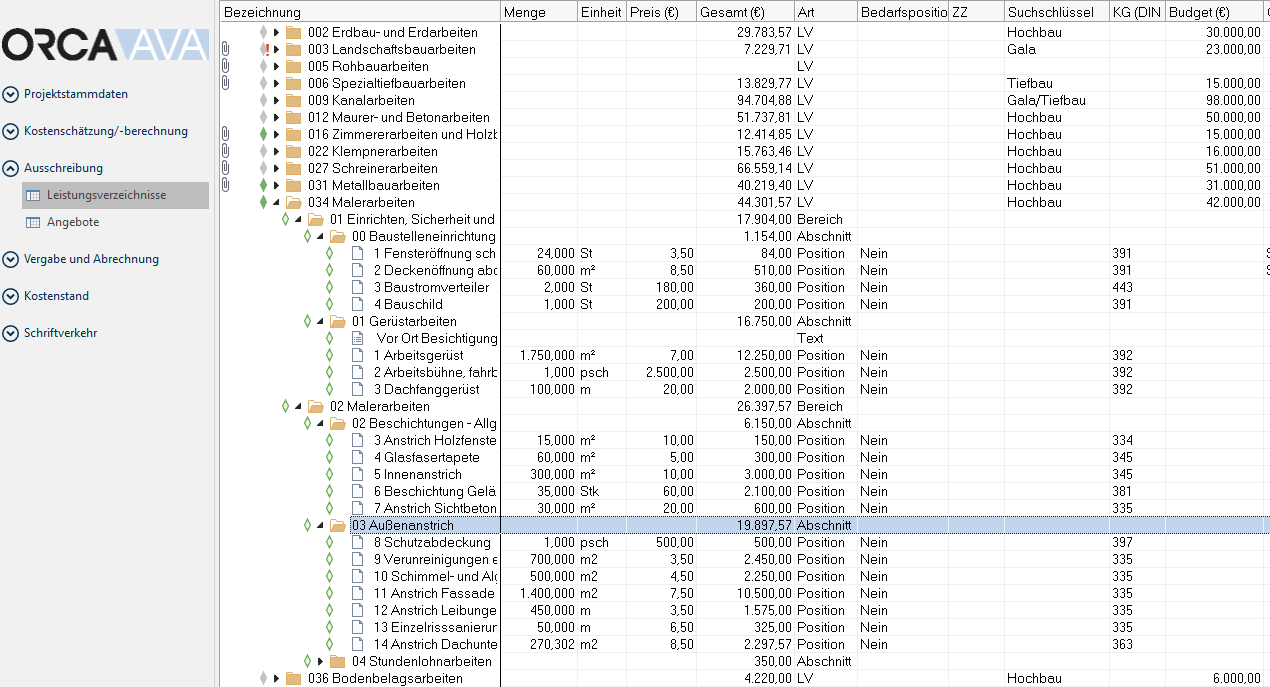
\includegraphics[width=1\textwidth]{\figdir/orca-ava-tree}}
%\end{figure}

\begin{figure}[b!]
	{\caption{Welche IT-Projekte haben in Ihren Unternehmen die höchste Priorität}
		\label{FIG:statistic-it-projects}}
	{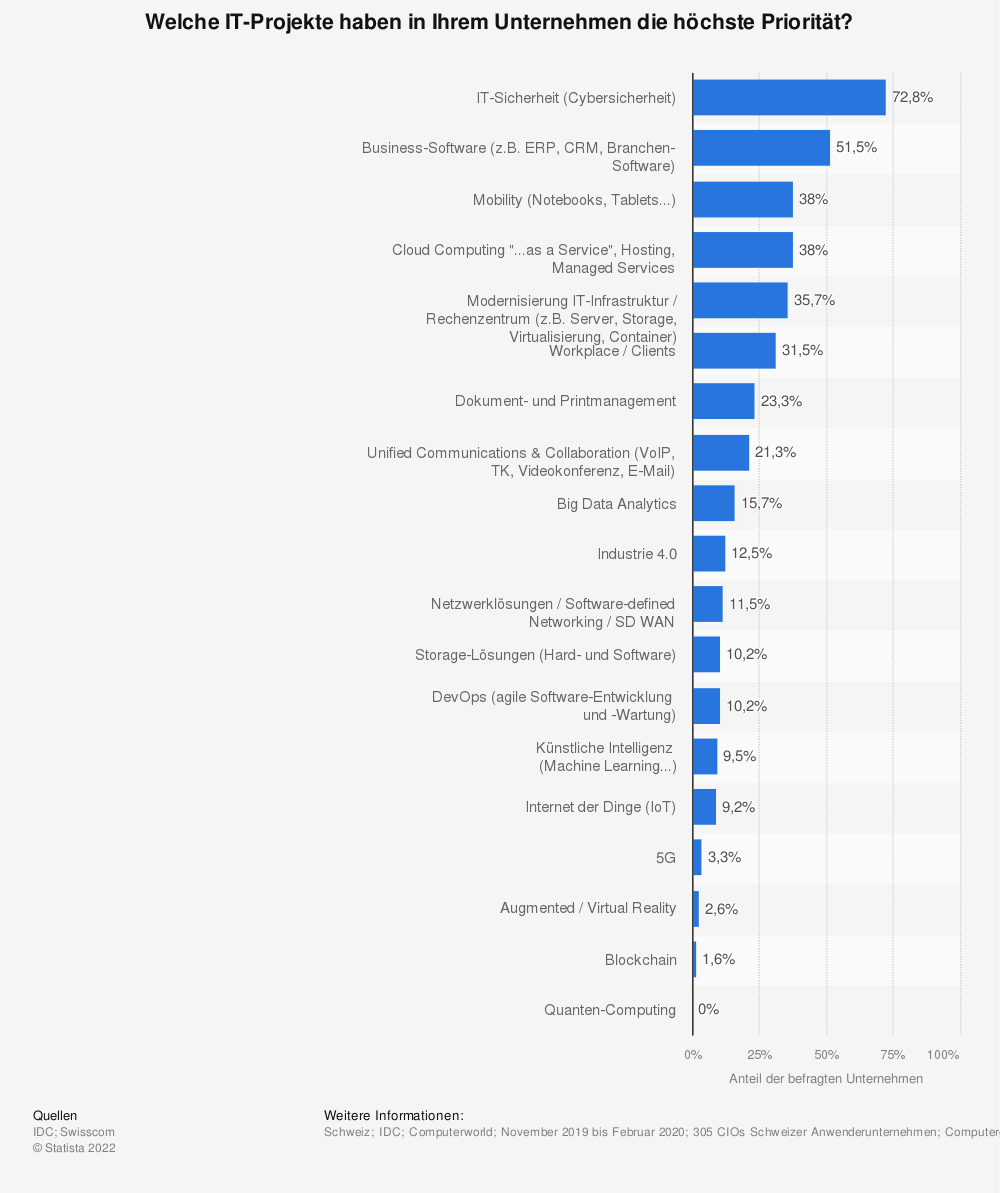
\includegraphics[width=1\textwidth]{figures/statistic-it-projekte.png}}
\end{figure}

\begin{figure}[b!]
	{\caption{Breakdown of software development methodologies practiced wordlwide in 2021}
		\label{FIG:devops-important}}
	{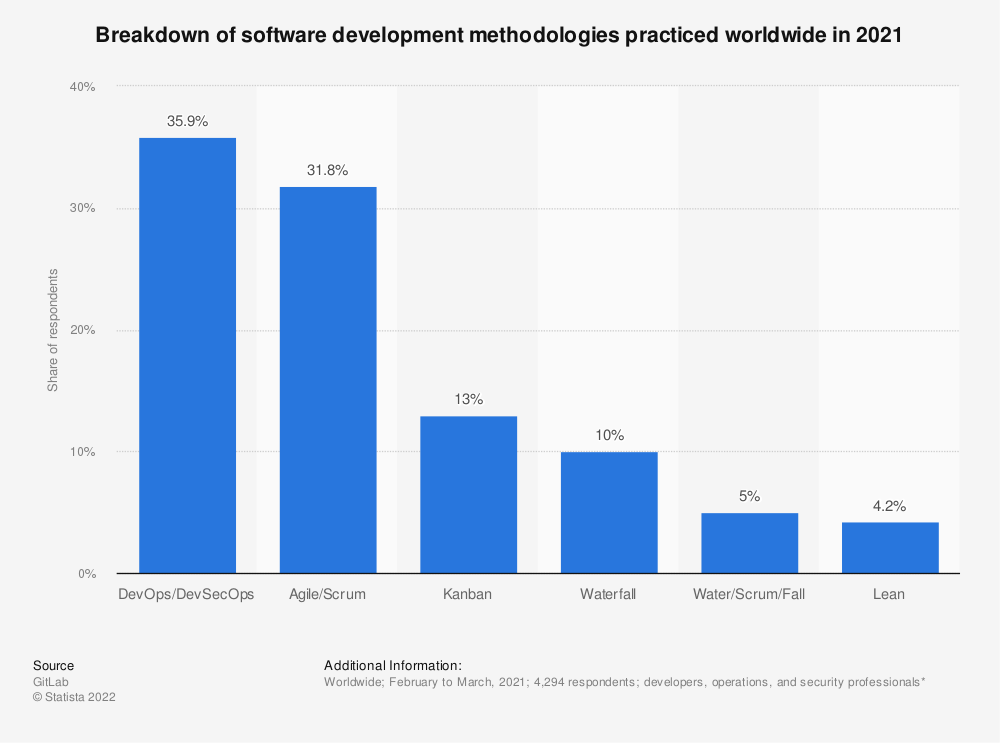
\includegraphics[width=1\textwidth]{figures/devops-important.png}}
\end{figure}

\begin{figure}[b!]
	{\caption{StackOverflow Trends von Github und Azure DevOps vom 18.06.2022}
		\label{FIG:github_azuredevops}}
	{  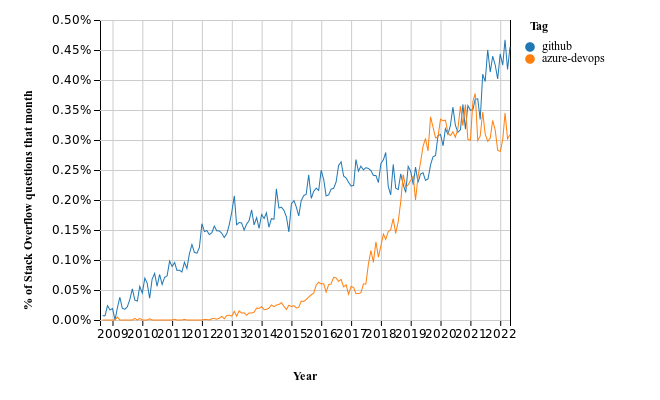
\includegraphics[width=1\textwidth]{figures/github_azuredevops.png}
	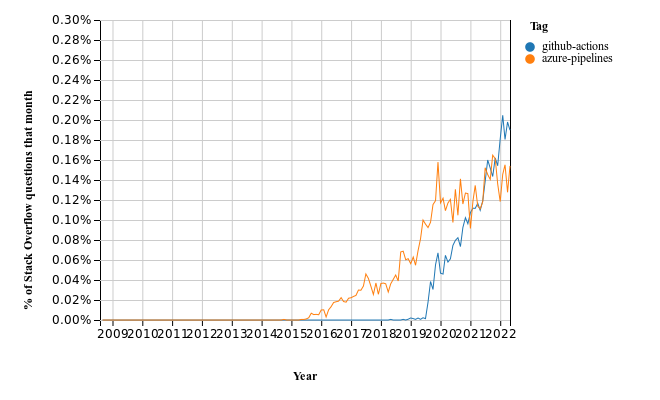
\includegraphics[width=1\textwidth]{figures/githubactions_azurepipelines.png}}
\end{figure}


%%% Local Variables: 
%%% mode: latex
%%% TeX-master: "thesis.tex"
%%% End: 


\cleardoublepage

\bibliographystyle{natger}
\bibliography{thesis}

\cleardoublepage

\footnotesize
\printindex

\pagenumbering{gobble}
{
	\large
	\thispagestyle{empty}
	\vspace*{\fill}
	
	\noindent
	\textsc{Eigenständigkeitserklärung / Declaration of Originality}
	
	\medskip
	
	\noindent
	Hiermit bestätige ich, dass ich die vorliegende Arbeit selbständig verfasst und keine anderen als die angegebenen Hilfsmittel benutzt habe. Die Stellen der Arbeit, die dem Wortlaut oder dem Sinn nach anderen Werken (dazu zählen auch Internetquellen) entnommen sind, wurden unter Angabe der Quelle kenntlich gemacht.
	
	\medskip
	
	\textit{I declare that I have authored this thesis independently, that I have not used other than the declared sources / resources, and that I have explicitly marked all material which has been quoted either literally or by content from the used sources.}
	
	\bigskip
	
	\noindent
	Rosenheim, den tt.mm.jjjj
	
	\vspace*{2cm}
	
	\noindent
	Vor- und Zuname
}

%%% Local Variables: 
%%% mode: latex
%%% TeX-master: "d"
%%% End: 



\end{document}
